\PassOptionsToPackage{dvipsnames}{xcolor}
\documentclass[12pt]{article}
%\documentclass[10pt,draft]{article}
\usepackage[utf8]{inputenc} % utf8 support

% === Document Layout ===
\usepackage[hmargin=0.75in,vmargin=0.75in]{geometry}
\usepackage{indentfirst}
\usepackage{lipsum}
\usepackage{url}
\usepackage[
    colorlinks,
    linkcolor=red!50!black,
    citecolor=blue!50!black,
    urlcolor=blue!50!black
]{hyperref}
\usepackage{amsmath}
\usepackage{pdfpages}
\usepackage{physics}
\usepackage{mathtools}
\usepackage{graphicx}
\usepackage{xcolor}
\usepackage{mathtools} % for the coloneq command
\usepackage{xparse}
\usepackage{ifthen} % For checking optional parameters
\usepackage{enumerate}
\usepackage{amsthm} % The AMS theorems package
\usepackage{amsthm}
\usepackage{caption}
\captionsetup{width=0.8\textwidth}
\usepackage{subcaption}
\usepackage{float}
\usepackage{tabularx}
\usepackage{authblk} % For affiliations
\usepackage{amsfonts}
\usepackage{indentfirst}
\usepackage{amssymb} % for ordering symbols
\usepackage{colonequals} % for the \ratio command

% amsthm
\newtheorem{theorem}{Theorem}[section]
\newtheorem{lemma}[theorem]{Lemma}
\newtheorem{proposition}[theorem]{Proposition}
\newtheorem{corollary}[theorem]{Corollary}
\newtheorem{conjecture}[theorem]{Conjecture}
\theoremstyle{definition}
\newtheorem{definition}{Definition}[section]
\theoremstyle{remark}
\newtheorem{remark}{Remark}

% === Bibliography ===
\usepackage[
    backend=biber,
    style=authoryear,
    citestyle=authoryear,
]{biblatex}
\addbibresource{references.bib}

\newcommand{\speccite}[1]{\citetitle{#1} \parencite{#1}}

\newcommand{\dt}[1]{\frac{\mathrm d #1}{\mathrm d t}}
\usepackage{pgfplots}
\usepackage{tikz}
\usepackage{tikz-3dplot}
\usetikzlibrary{calc}
\tikzset{every picture/.style={baseline={(current bounding box.center)}}}

\author[1,2]{Thomas C. Fraser}
\affil[1]{Perimeter Institute for Theoretical Physics, Waterloo, Ontario, Canada, N2L 2Y5}
\affil[2]{Dept. of Physics and Astronomy, University of Waterloo, Waterloo, Ontario, Canada, N2L 3G1}
\date{\today}

\title{On the Causality of Dynamical Systems}

\begin{document}
\maketitle

\section*{Comments}

These notes can be found at \url{https://github.com/tcfraser/pearl_and_dynamic_causality}. \\

\section{A Chaotic Origin Story}

\subsection{Lorenz's Discovery}
In \speccite{lorenz1963deterministic}, \citeauthor{lorenz1963deterministic} (this is Edward Norton Lorenz, not to be confused with the physicist Ludvig Lorenz, or the actor Edward Norton) presented a simplified dynamical model for atmospheric convection, which today is known as the Lorenz system:
\begin{align}
    \begin{split}
        \dt{X} &= \sigma ( Y - X ), \\
        \dt{Y} &= X ( \rho - Z ) - Y, \\
        \dt{Z} &= XY - \beta Z.
    \end{split}
\end{align}
The Lorenz system was remarkable because despite its determinism and simplicity, it exhibits flows which are non-periodic, chaotic and yet bounded as in Figure~\ref{lorenz_system}. Moreover, Lorenz identifies the non-linearity of the equations as being essential for these features postulates their ubiquity.
\begin{figure}[H]
    \centering
    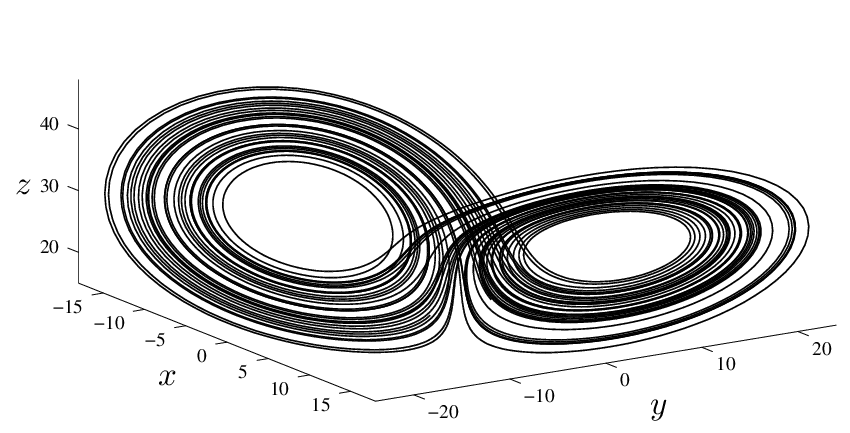
\includegraphics[scale=0.35]{figures/lorenz_system.png}
    \caption{The strange attractor of the Lorenz system for $\sigma = 10, \beta = 8/3, \rho = 28$ with $X(0) = 1.1, Y(0) = -1.9, Z(0) = 13.1$. Figure by \href{https://www.researchgate.net/figure/A-trajectory-of-the-Lorenz-system-in-phase-space-revealing-the-strange-attractor-The_fig1_262074522}{P. T. Clemson}.}
    \label{lorenz_system}
\end{figure}

Later in \speccite{ruelle1971nature}, \citeauthor{ruelle1971nature} develop a variety of mathematics to study such quasi-periodic behaviors and refers to them as \textit{strange attractors}. Importantly, they conjectured that universally, strange attractors where the cause of turbulent behaviors seen in fluid flow. This conjecture received further support after \speccite{gollub1975onset}.

\subsection{What are attractors anyway?}
What exactly is notion of an \textit{attractor}? Intuitively, attractors generalize the more familiar notions of stability for differential equations such as \textit{stable fixed points} and \textit{limit cycles} in the sense that an attractor $A$ is a compact subset such that points starting sufficiently close to $A$ will remain in a given neighborhood of $A$. For a detailed account of the various notions and formulations of an attractor, see \speccite{milnor1985concept}. Nevertheless, the following definition will be adequate.

A dynamical system on a manifold $M$ (for example $\mathbb R^n$) is specified by a \textbf{flow} (a solution to the system of ODEs)
\begin{equation}
    \Phi_{(\cdot)}(\cdot) : \mathbb R \times M \to M,
\end{equation}
where $\Phi_t$ is a diffeomorphism of $M$ for all $t \in \mathbb R$ such that
\begin{equation}
    \forall V \in M : \Phi_{0} ( V ) = V, \quad \text{and} \quad \forall s,t \in \mathbb R: \Phi_t \circ \Phi_s = \Phi_{s+t}.
\end{equation}
An \textbf{attractor} is any $A \subseteq M$ which is
\begin{enumerate}
    \item forward invariant
        \[ \forall a \in A, \forall t \geq 0 : \Phi_{t} ( a ) \in A, \]
    \item admits an neighborhood $B(A)$, called the \textbf{basin of attraction}, such for every open neighborhood $N$ of $A$, there is a sufficiently large $T$ such that
        \[ \forall b \in B(A), \forall t \geq T : \Phi_{t} ( b ) \in N, \]
    \item and finally, there is no other proper subset $A' \subset A$ satisfying the above.
\end{enumerate}
Note that some alternative definitions demand that $A$ has non-zero measure (i.e. to eliminate stable fixed points) or that there exists a orbit of the flow that is dense inside $A$.

What makes a strange attractor so \textit{strange}? At the time, \citeauthor{ruelle1971nature} never articulated a concrete definition for strange attractors, instead is was simply an attractor that was ``strange'' to them. Today, strange attractors are defined to be attractors whose dimension is not an integer, i.e. a fractal. Of course, the Lorenz attractor is a strange attractor in this sense as well, as proven in \speccite{tucker2002rigorous}.

\begin{figure}[H]
    \centering
    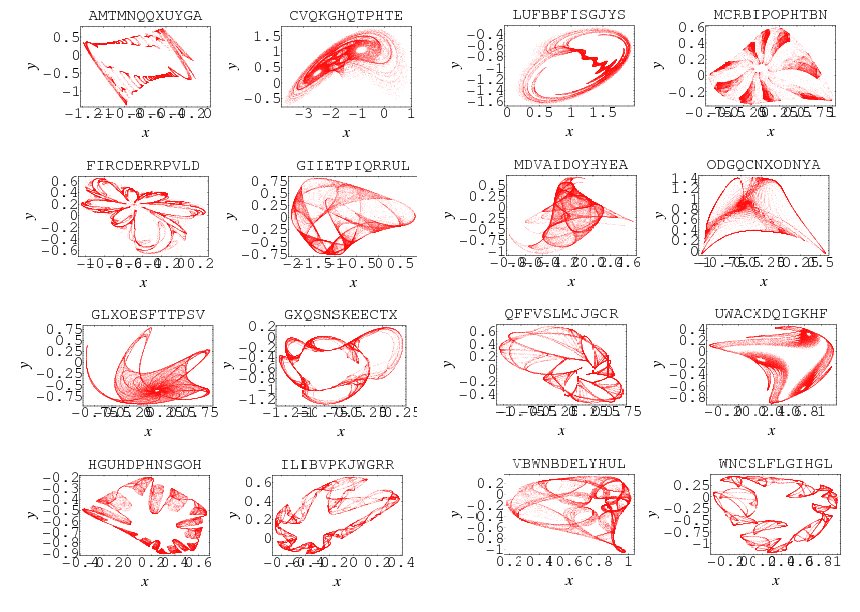
\includegraphics[scale=0.6]{figures/strange_attractors.png}
    \caption{Some strange attractors. Figures from \href{http://mathworld.wolfram.com/StrangeAttractor.html}{E. W. Weisstein}.}
\end{figure}

\subsection{Reconstructing Attractors}
In \speccite{packard1980geometry}, \citeauthor{packard1980geometry} were interested in problem of \textit{dynamical reconstruction}: from experimental observations of a turbulent fluid flow, how does one show the existence of a low-dimensional chaotic dynamical system which explains the observed behaviors? Additionally, how does one determine the dimensionality of the underlying attractor? They demonstrate their ideas using another non-linear dynamical system studied by \parencite{rossler1976equation}:

\begin{align}
    \label{rossler}
    \begin{split}
        \dt{X} &= - ( Y + Z ), \\
        \dt{Y} &= X + 0.2 Y, \\
        \dt{Z} &= 0.4 + XZ - 5.7 Z.
    \end{split}
\end{align}

Their reconstruction method relied directly on the intuition that in order to specify the state of an $n$-dimensional system at any given time, it is sufficient to known the values of \textit{any} set of $n$ ``independent'' quantities. Moreover, they conjecture that the attractors associated with any such are all \textit{diffeomorphically} equivalent. To support this claim, they compare various trajectories in $3$-dimensions of the Rossler system: $\{ X(t), Y(t), Z(t)\}$, $\{ X(t), X(t - \tau), X(t - 2 \tau)\}$ (this example is credited to Ruelle by the authors), and $\{ X(t), \dot X(t), \ddot X(t) \}$ (by making $\tau$ very small and taking appropriate differences).

\begin{figure}[H]
    \centering
    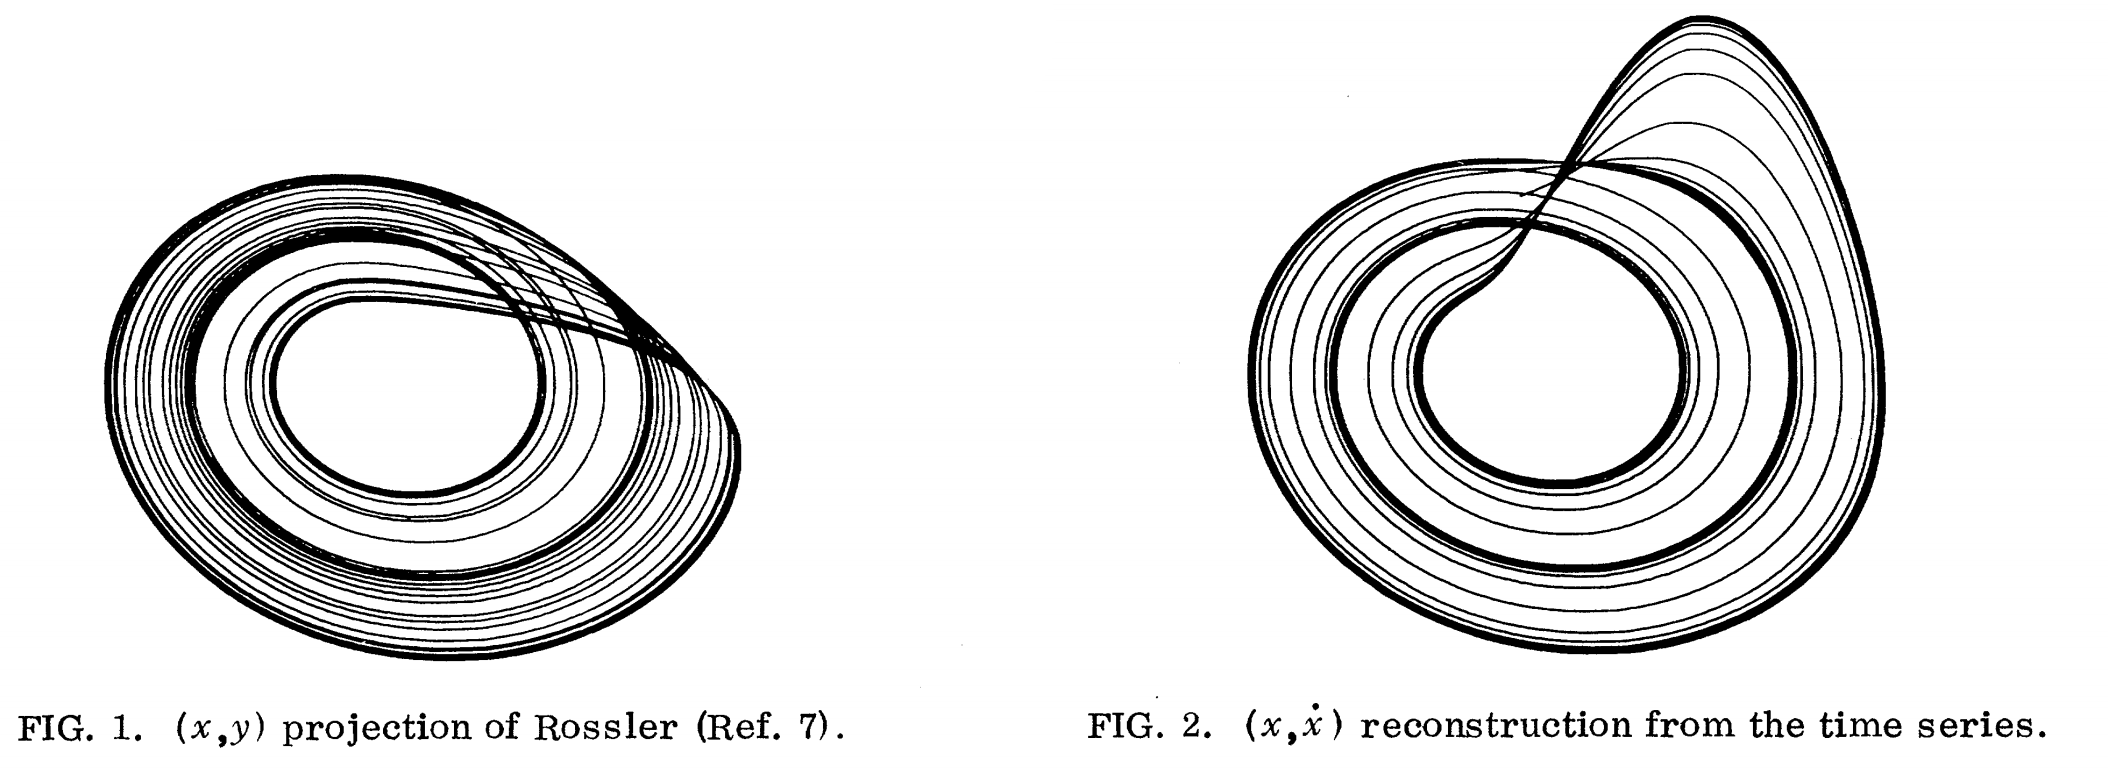
\includegraphics[scale=0.25]{figures/rossler_reconstruction.png}
    \caption{The \citeauthor{rossler1976equation} system flow projected onto the $X, Y$ plane and the induced flow of $(X, \dot X, \ddot X)$ projected onto the $X, \dot X$ plane. Figure from \parencite{packard1980geometry}.}
\end{figure}

Evidently their heuristic seems to work and moreover it appears possible to reconstruct the dynamics from observing just a single coordinate. They further provide some tools for estimating the dimensionality of the attractor and how it relates to the number non-negative characteristic exponents.

\subsection{Takens' Theorem}

Shortly after this, in \speccite{takens1981detecting}, \citeauthor{takens1981detecting} formalized and proved the conjecture of \parencite{packard1980geometry} which has come to be known as \textit{Takens' Theorem}. The following is a summary of \href{https://www.math.sciences.univ-nantes.fr/~vitturi/talks/PG%20Colloquia/Takens_theorem.pdf}{Marco Vitturi's slides} on the subject.

\textbf{Whitney Embedding Theorem:}
Let $M$ be a compact manifold of (integer) dimension $d$. Then $M$ can be embedded smoothly in $\mathbb{R}^{2n}$ (i.e. no self-intersections).

\begin{figure}[H]
    \centering
    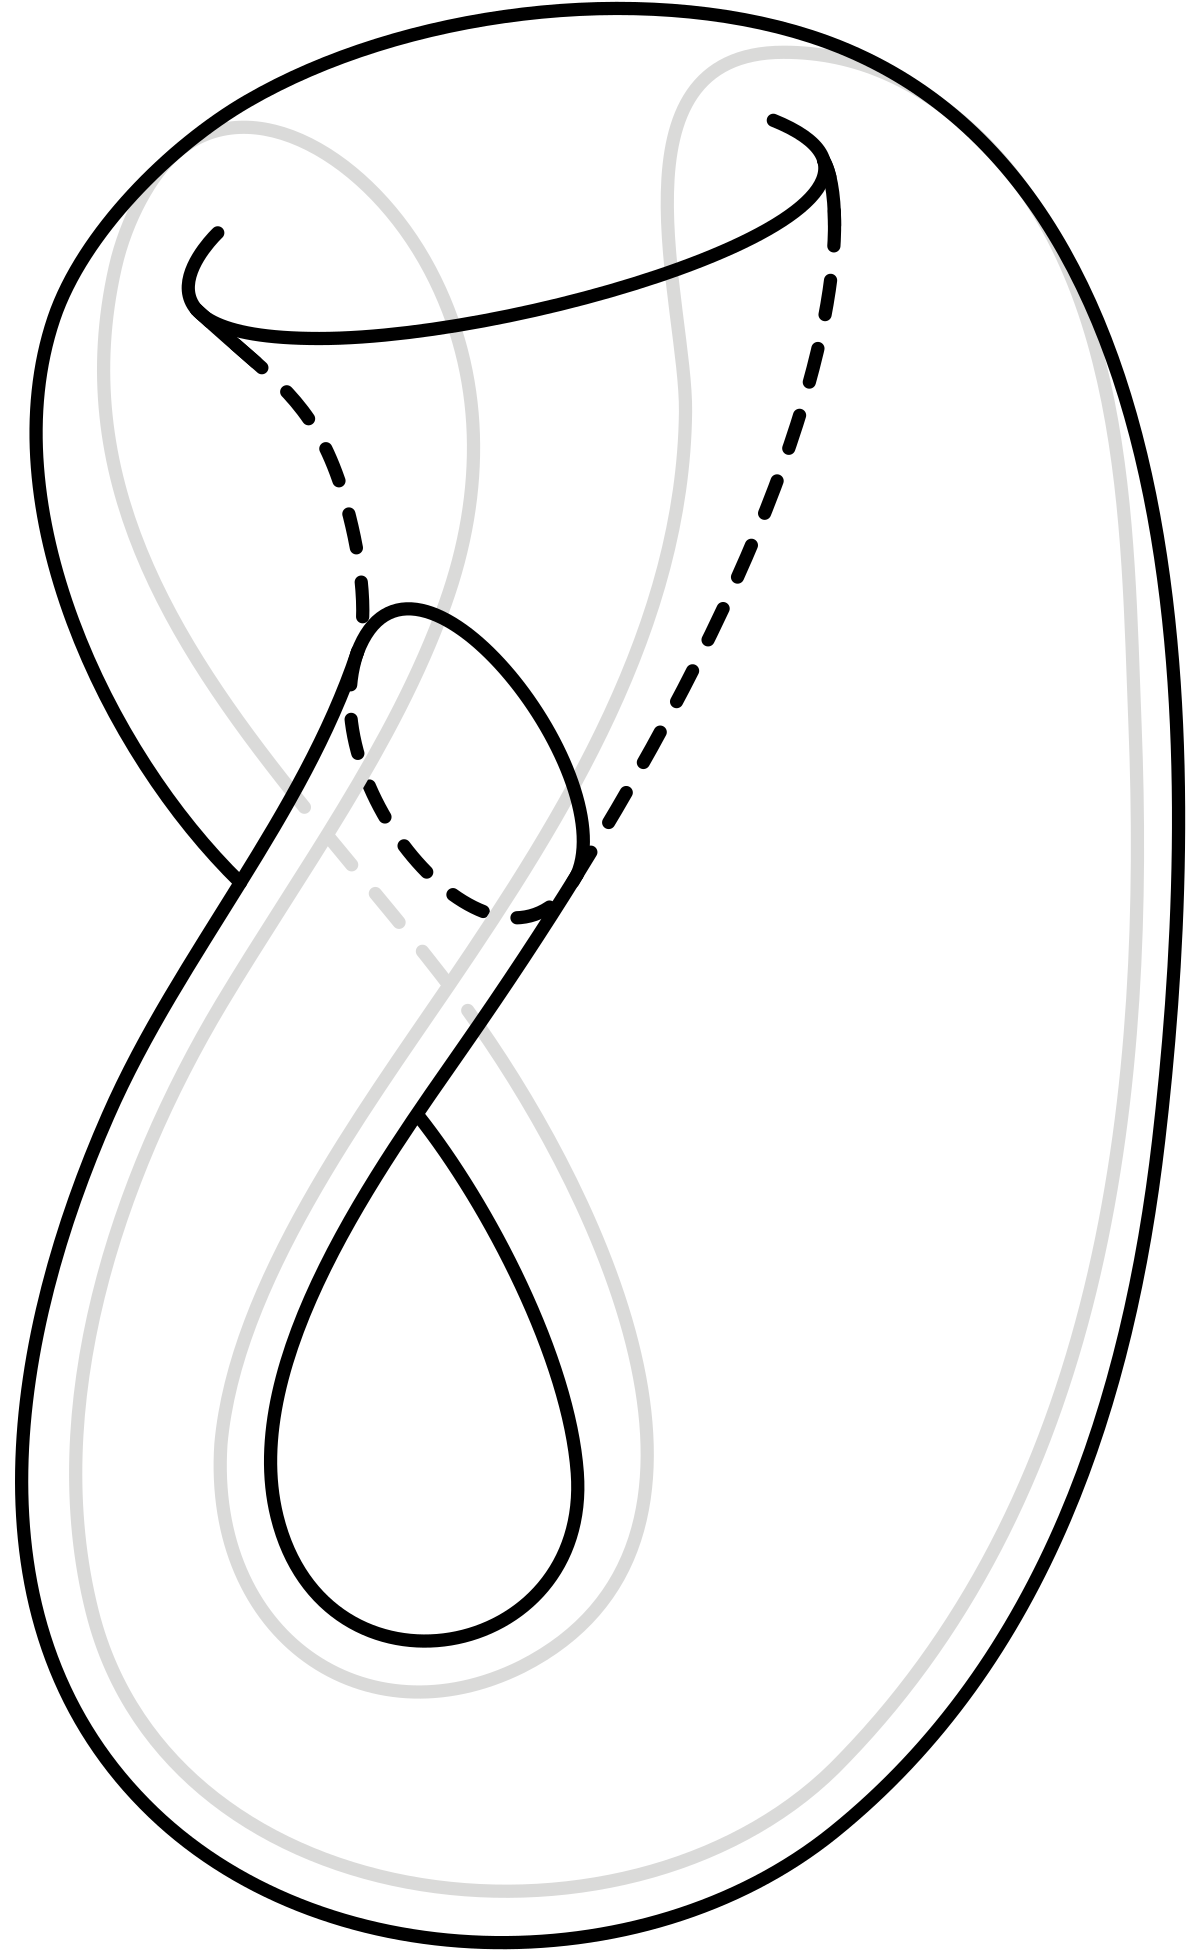
\includegraphics[scale=0.1]{figures/klein_bottle.png}
    \caption{The Klein bottle can be embedded smoothly in $\mathbb R^4$, but not in $\mathbb R^3$.}
\end{figure}

\textbf{Takens' Theorem:}
Let $M$ be a compact manifold of (integer) dimension $d$. Then for \textit{generic} pairs $(\phi, X)$, where
\begin{itemize}
    \item $\phi : M \to M$ is a $C^2$-diffeomorphism of $M$ in itself,
    \item $X : M \to \mathbb R$ is a $C^2$-differentiable function,
\end{itemize}
then the map $\Omega_{\phi, X} : M \to \mathbb R^{2d + 1}$ acting on $V \in M$ defined by
\[ \Omega_{\phi, X}(V) = ( X(V), X(\phi(V)), X(\phi^2(V)), \cdots, X(\phi^{2d}(V))) \]
is an embedding of $M$ into $\mathbb{R}^{2d+1}$ (i.e. injective and immersive).

Takens' theorem when applied to the flow of a dynamical system in $\mathbb R^n$ when $M$ is taken to be the attractor (assume manifold) $A$:
\begin{itemize}
    \item $\phi = \Phi_{-\tau} : A \to A$ for some $\tau > 0$,
    \item $X : A \to \mathbb R$ any coordinate of the system on the attractor,
    \item the \textbf{delay embedding} becomes
        \begin{align*}
            \Omega_{\Phi_{-\tau}, X}(V)
            &= ( X(V), X(\Phi_{-\tau}(V)), X(\Phi_{-2\tau}(V)), \cdots, X(\Phi_{-m\tau}(V))) \\
            &= ( X(t), X(t - \tau), X(t - 2 \tau), \cdots, X(t - m \tau))
        \end{align*}
    \item where $m$ needs to be sufficiently large, i.e. $m \geq 2 \mathrm{dim} (A)$ is sufficient.
    \item Oftentimes a smaller $m$ will still produce an embedding, but Takens' theorem does not guarantee this.
\end{itemize}
A similar result can be stated for reconstructing the orbit in $\mathbb{R}^d$ instead of the entire attractor, you can use $m = d - 1$. Therefore a single variable contains all the information about the orbit:
\[ t \mapsto ( X(t), X(t - \tau), X(t - 2 \tau), \cdots, X(t - (d-1) \tau)). \]

An analogous version for the case of non-integer (Hausdorff) dimensions $d_A$ is due to \speccite{sauer1991embedology}, where $m \geq \lceil 2 d_{A} \rceil}$.

Therefore, the attractor $A$ of the original system is diffeomorphic to the time-delayed attractors $A_X, A_Y$ and $A_Z$ where $A_X = \Omega_{\Phi_{-\tau}, X}(A)$.

Evidently, Takens' theorem reveals that the distinction between the kinematics and dynamics of a system is an arbitrary distinction as one can freely transform between the various phase-spaces in a diffeomorphic way. For similar instances of this arbitrary distinction, and more ideas on this subject, see \speccite{spekkens2015paradigm}.

\section{Selected References on Dynamic Causality}

\subsection{Granger Causality}

There is a pervasive notion of causality used frequently in economic forecasting, but also in neurology and ecology, known as \textit{Granger Causality} or sometimes \textit{G-Causality} named after Clive Granger. For evidence, the library of software tools \speccite{barnett2014mvgc} is highly cited.  Its origins can be traced back to a suggestion due to (Wiener, 1956) for using prediction as a proxy for causality, which was subsequently developed by Granger from 1963 to 1980. Granger was awarded the Novel Prize in Economics in 2003.

In \speccite{granger1988some}, \citeauthor{granger1988some} summarizes his notions of causality for time-series' which were based on two principles:
\begin{enumerate}
    \item The cause occurs before the effect.
    \item The causal series (say $Y(t)$) contains \textit{special information} about the series being caused (say $X(t)$) that is not available in the any other available series (say $W(t)$).
\end{enumerate}

Consider two sets of historical data:
\begin{align}
    J_t &= \{ (X(t-j), Y(t-j), W(t-j)) | j \geq 0 \} \\
    J_t' &= \{ (X(t-j), W(t-j)) | j \geq 0 \}.
\end{align}
His definitions pertain to the following: in the context of $W$, does $Y$ cause $X$?

Letting $P(X | J)$ denote the conditional distribution of $X$ given $J$, if $P(X(t+1) | J_t) = P(X(t+1) | J_t')$ then $Y(t)$ does \textit{not cause} $X(t)$, otherwise $Y(t)$ is a \textit{prima facie cause} of $X(t)$ and becomes a cause with certainty is $J_t$ contains all the information in the universe. Granger acknowledges a number of criticisms in his works.

Most relevant for the current discussion is the article \speccite{lusch2016inferring}, which simulated network systems of Kuramoto oscillators and then used the MGVC toolbox to reconstruct the network structure. They write ``Our results show a significant systematic disparity between the original and inferred network, unless the true structure is extremely sparse or dense.''

\begin{figure}[H]
    \centering
    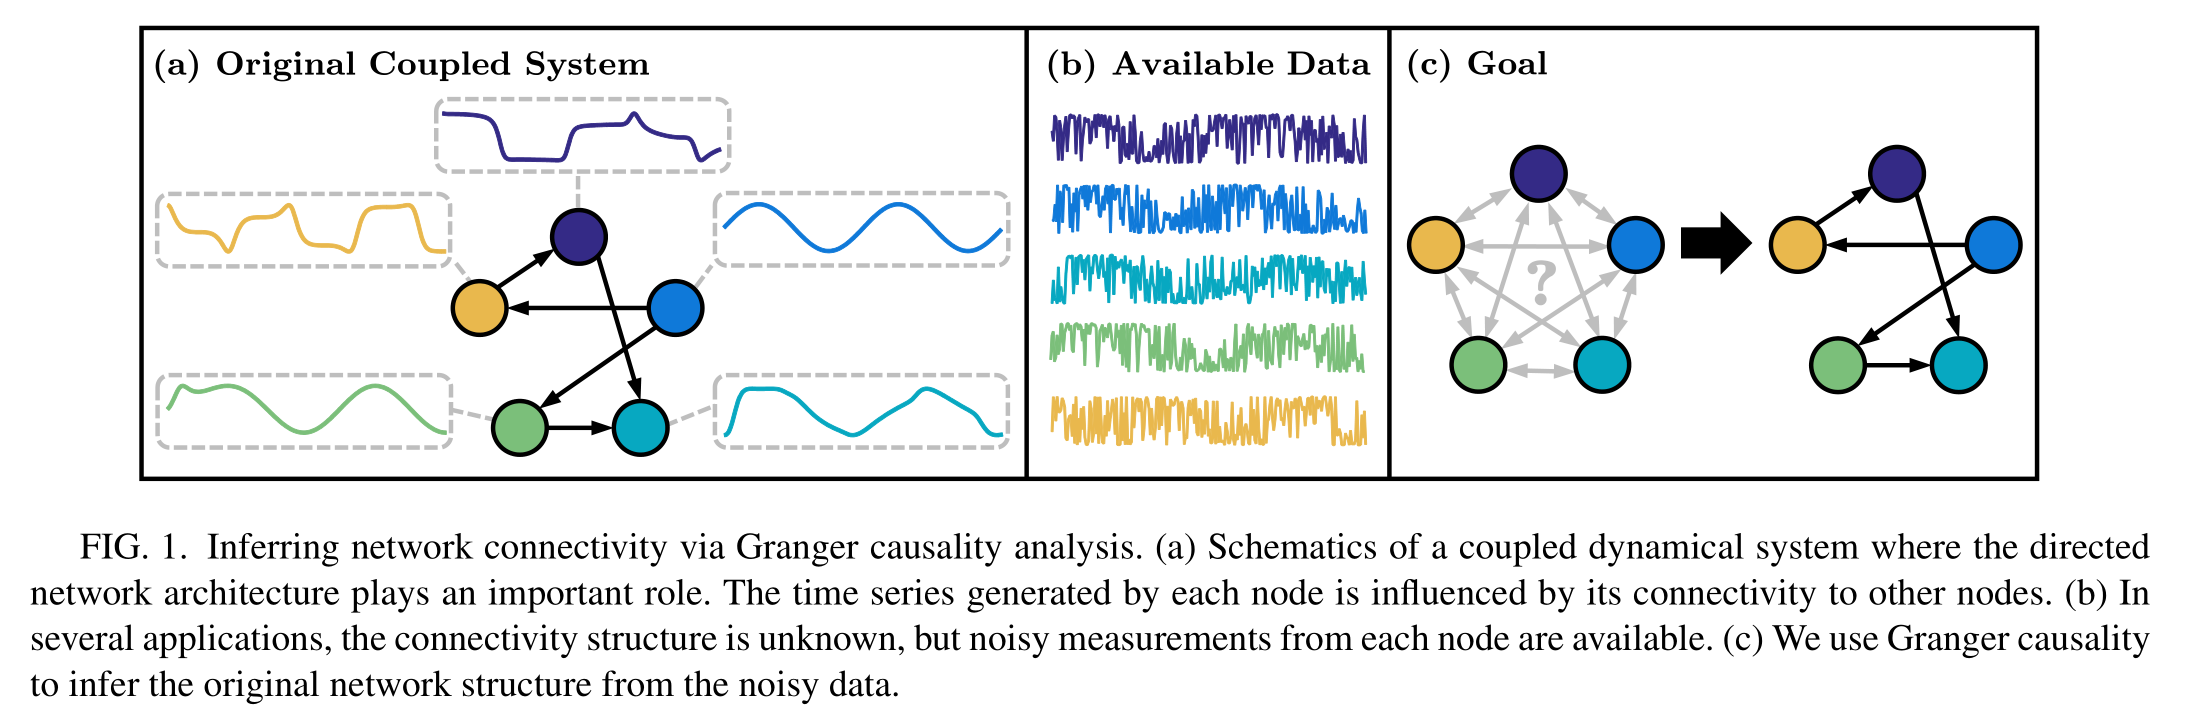
\includegraphics[scale=0.3]{figures/granger_reconstruction.png}
    \caption{The methodology used by \speccite{lusch2016inferring}.}
\end{figure}

Clearly, Granger's notions of causality are inappropriate for the purposes of causal modeling, despite its widespread use.

\subsection{Convergent Cross Mapping (CCM)}

The seminal article titled \speccite{sugihara2012detecting} has been widely cited in other articles on dynamical causality and throughout ecological and economic communities. Its essential accomplishment, in my opinion, was the realization that nonlinear dynamical systems exhibit a kind of nonseparability which must be dealt with first in order analyze the underlying causal relations and moreover that Takens' theorem resolves this nonseparability.

It opens with an discussion around the notions of ephemeral or ``mirage'' correlations. The following discrete-time non-linear dynamical system,
\begin{align}
    \label{ecosystems}
    \begin{split}
        X(t+1) &= X(t) ( r_x - r_x X(t) - \beta_{x,y} Y(t) ) \\
        Y(t+1) &= Y(t) ( r_y - r_y Y(t) - \beta_{y,x} X(t) )
    \end{split}
\end{align}
exhibits periods of correlation, anticorrelation and no correlation.
\begin{figure}[H]
    \centering
    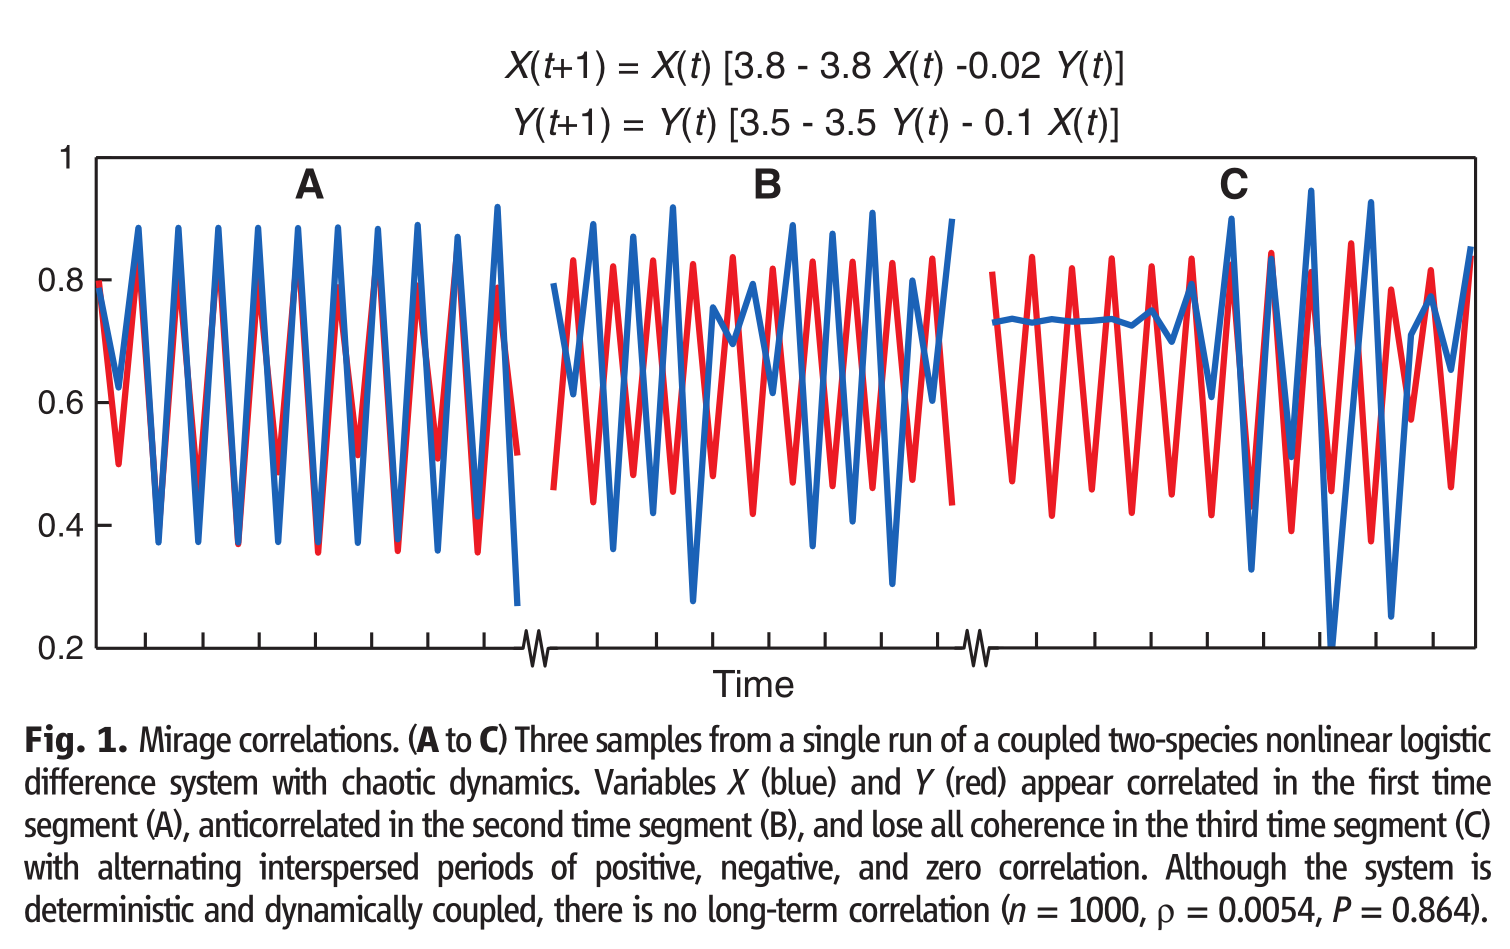
\includegraphics[scale=0.35]{figures/mirage_correlations.png}
    \caption{An illustration of mirage correlations from \speccite{sugihara2012detecting}.}
\end{figure}
Therefore, using correlation to infer causation is risky, especially in nonlinear dynamics. Moreover, this demonstrates why a lack of correlation does not imply a lack of causation because the former could simply be temporary. In other words, the principle of no fine-tuning only applies in the long term.

\citeauthor{sugihara2012detecting} attributes the inadequacy of Granger causality for dynamical systems to Takens' theorem. In particular, ``information about $X(t)$ that is relevant to predicting $Y$ is redundant in this system''. Stated another way, by algebraically rearranging Eq.~\ref{ecosystems}, it is possible to write $Y(t+1)$ in terms of $Y(t)$ and $Y(t-1)$; thus Granger causality predicts $X$ does not cause $Y$! In \speccite{harnack2017topological}, this nonseparability is referred to as an \textit{entanglement} between $X$ and $Y$.

The essential idea of \parencite{sugihara2012detecting} is that time-series variables $X$ and $Y$ are \textit{causally linked} if they share a common attractor manifold $A$; therefore, each variable can identify the other. Convergent cross mapping (CCM) tests for causal influence from $X$ to $Y$ by measuring the extent to which the history of $Y$ can reliably estimate the states of $X$. For example, a fish time series $Y$ can be used to estimate the weather $X$, but not conversely, thus $X$ causes $Y$; this is counter to Granger causality.

\begin{figure}[H]
    \centering
    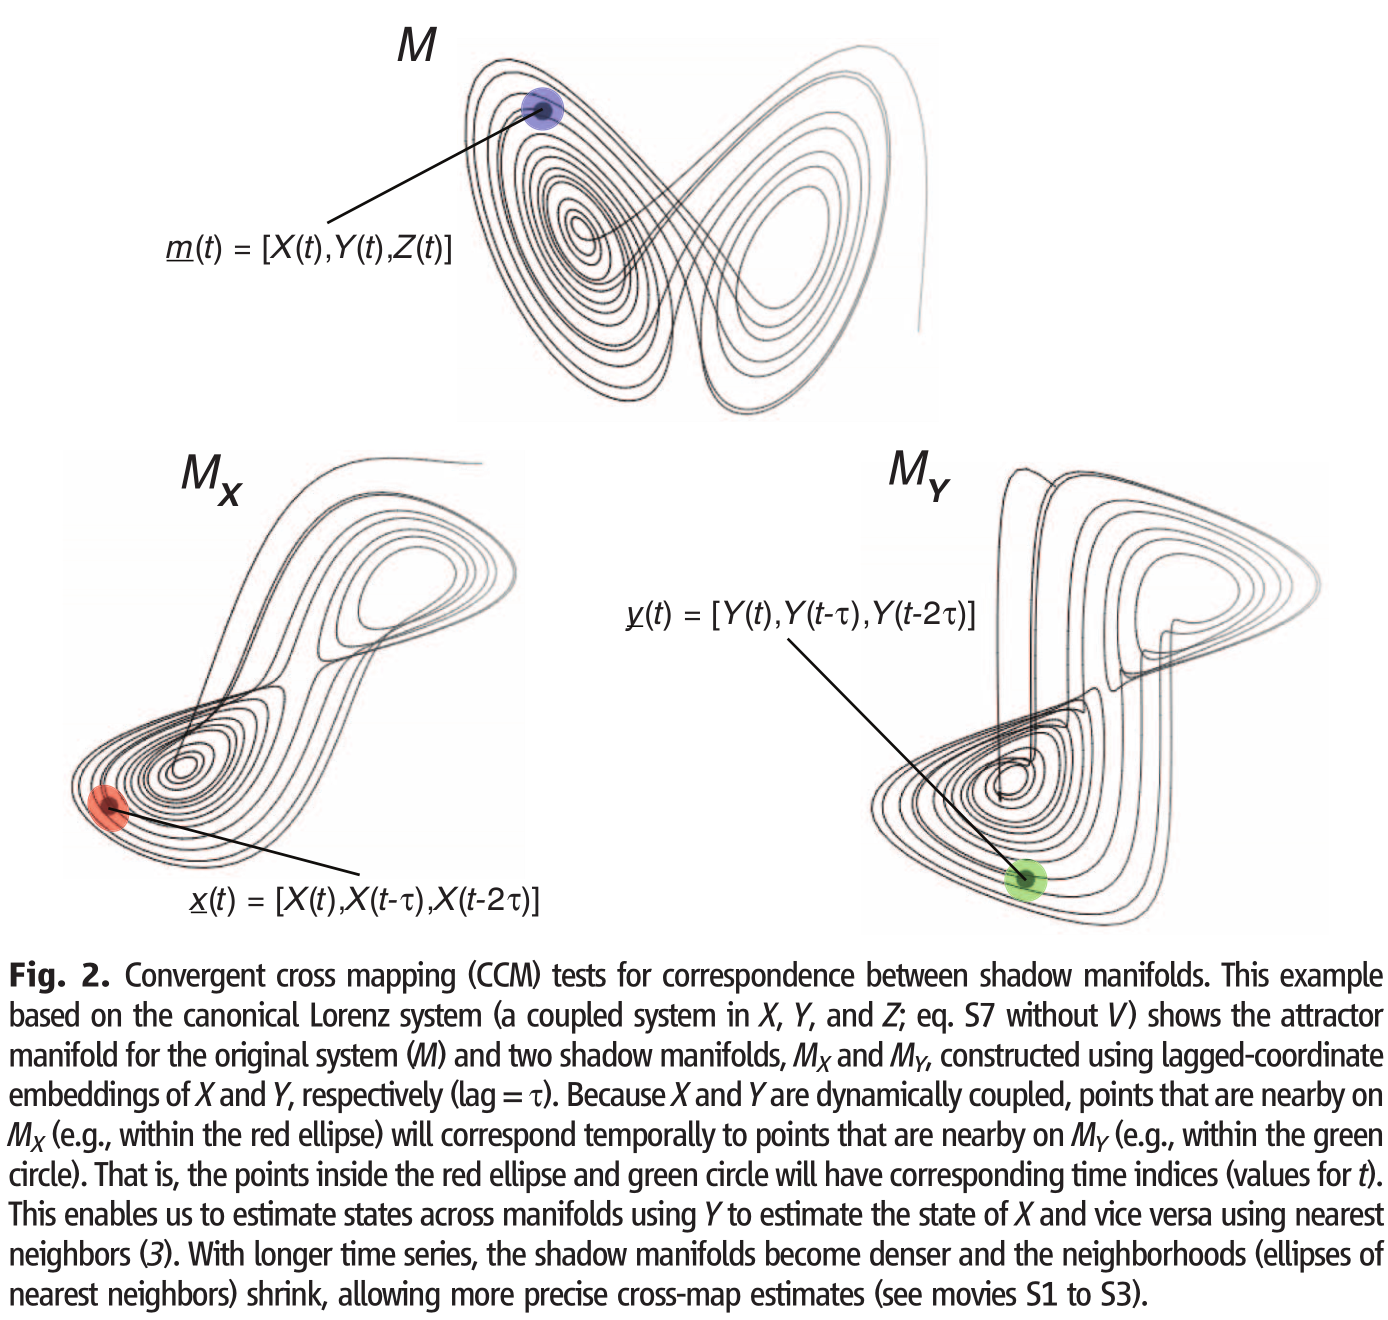
\includegraphics[scale=0.4]{figures/convergent_cross_mapping.png}
    \caption{The method of convergent cross mapping (CCM) due to \speccite{sugihara2012detecting}.}
\end{figure}

\textbf{Sketching the CCM Algorithm:}
\begin{enumerate}
    \item Given two time series of length $L$,
        \[ \{ X(1), X(2), \ldots, X(L) \} \quad \text{and} \quad \{ Y(1), Y(2), \ldots, Y(L) \}, \]
        here is how to estimate $Y(t)$ using $X$.
    \item Compute the time lagged coordinate
        \[ \underline{X}(t) = ( X(t), X(t - \tau), X(t - 2 \tau), \ldots, X(t-(d-1)\tau)\}. \]
    \item Then find its $d+1$ nearest neighbors in $A_{X}$, denoted
        \[ (\underline{X}(t_1), \underline{X}(t_2), \ldots, \underline{X}(t_{d+1}) ), \]
        thus forming a $d$-dimensional simplex around $\underline{X}(t)$.
    \item Construct the estimate $\hat Y(t)$ for $Y(t)$ as
        \[ \hat Y(t) | A_X = \sum_{i=1}^{d+1} \omega_{i} Y(t_i) \]
        where the weight $\omega_{i}$ is based on the distance between $\underline X(t)$ and $\underline X(t_i)$.
    \item As the length $L$ increases, the attractor manifold is filled in more and more, and the nearest neighbors get closer and thus $\hat Y(t) | A_X$ should converge to $Y(t)$ (if $Y$ has causal influence on $X$) and vice versa.
\end{enumerate}

\begin{figure}[H]
    \centering
    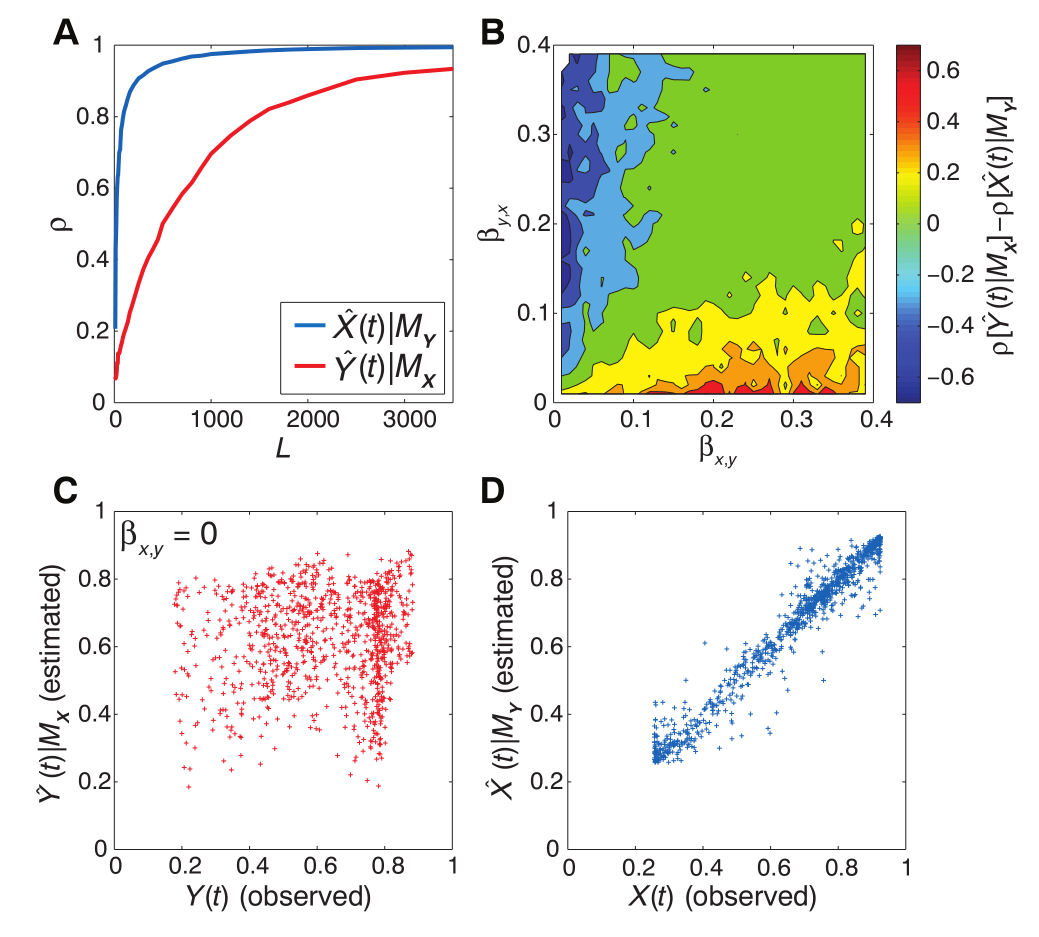
\includegraphics[scale=0.55]{figures/convergence.png}
    \caption{Empirical results for CCM on Eq.~\ref{ecosystems}. (A) CCM where $\beta_{y,x} > \beta_{x,y}$; the asymmetry is reflected in the differing rates of convergence. (B) How the difference in cross-mapping estimates depends on $\beta_{x,y}$ and $\beta_{y,x}$.   (C,D) Estimates when $\beta_{x,y} = 0$, i.e. when $Y$ has no effect on $X$. From \speccite{sugihara2012detecting}.}
\end{figure}

\begin{figure}[H]
    \centering
    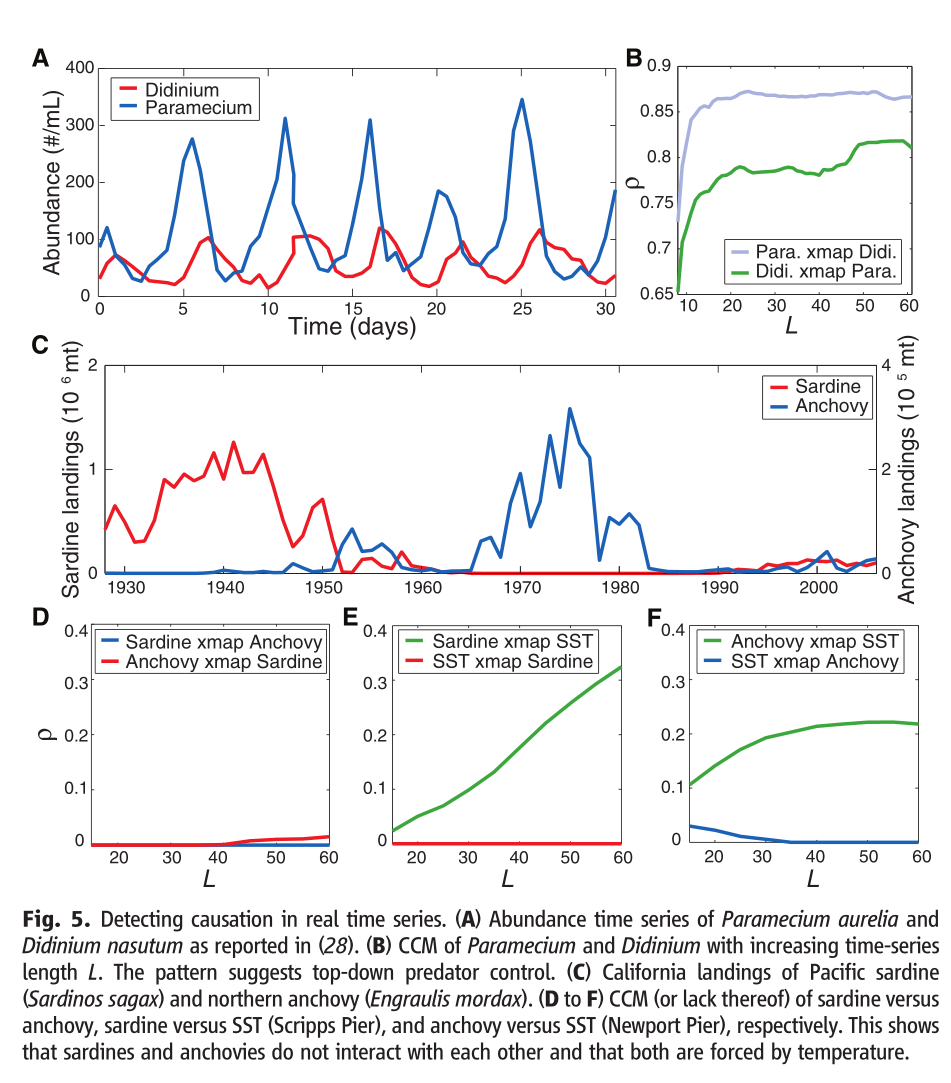
\includegraphics[scale=0.6]{figures/sardines_vs_anchovies.png}
    \caption{(C-F) CCM resolves a long-disputed causal relationship between populations of sardines and anchovies along with sea surface temperatures (SST) measured at Scripps Pier and Newport Pier in California; sardines and anchovies are not interacting, but share a common cause, namely SST. From \speccite{sugihara2012detecting}.}
\end{figure}

Future work demonstrated that CCM successfully distinguishes between direct and indirect causation in causal chains \parencite{ye2015distinguishing}.

\subsection{Topological Causality (TC)}

In \speccite{harnack2017topological}, the concepts of CCM are expanded upon further.
\begin{align*}
    \dt{X_1} &= f_1 ( X_1, w_{12} \mu_2 ( X_2 ) ) \\
    \dt{X_2} &= f_2 ( X_2, w_{21} \mu_1 ( X_1 ) )
\end{align*}
Theoretically, if the diffeomorphism between the attractor manifolds is differentiable, then it can be linearized at a fixed time $t$ (Jacobian matrix), denoted $M_{i\to j}^{t}$. The \textit{expansion} of this linear map, denoted
\[ e^{t}_{i \to j} = \prod_{k} \mathrm{max} (1, \sigma_{k} (M_{i\to j}^{t})) \]
is conjectured to be inversely proportional to the strength of the causal influence $X_j \to X_i$ ($\sigma_{k}(M_{i \to j}^{t})$ is the $k$-th singular value of $M_{i \to j}^{t}$). Unlike vanilla CCM, TC computes a \textit{graduated} measure causal influence which furthermore can be taken to be time-dependent.

\begin{figure}[H]
    \centering
    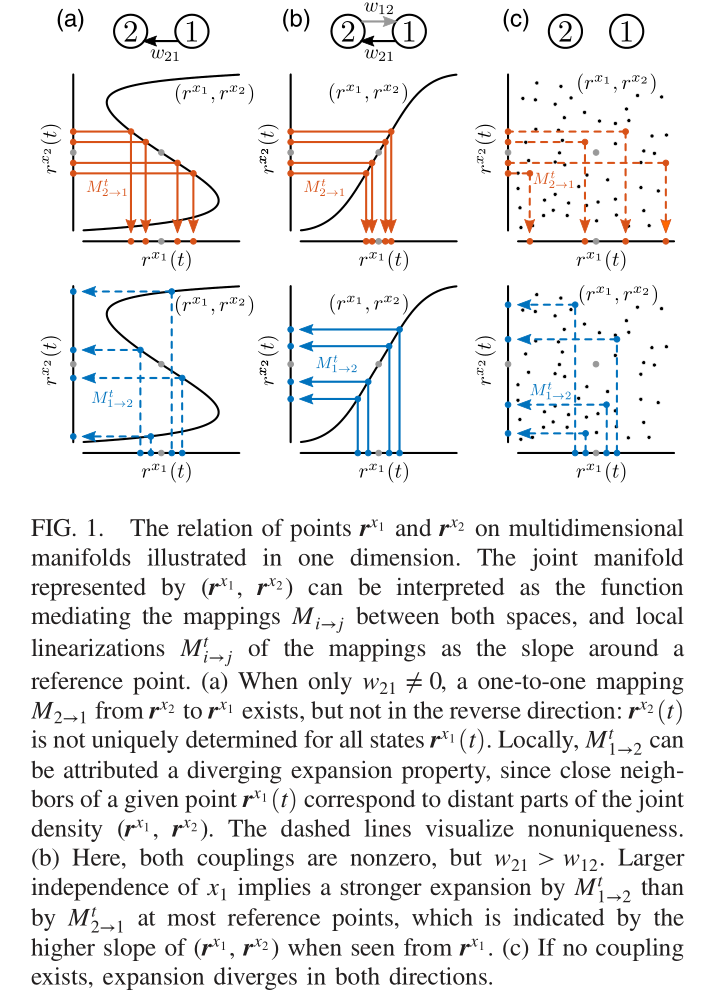
\includegraphics[scale=0.6]{figures/topological_causality.png}
    \caption{The intuition behind the inverse relationship between expansion and causal influence in \speccite{harnack2017topological}.}
\end{figure}

\subsection{Dimensional Causality (DC)}

The latest development in the field of dynamic causality based on Takens' theorem is the article \speccite{benkHo2018exact}, which presents a method called \textit{Dimensional Causality} (DC). While recognizing the utility of the CCM \parencite{sugihara2012detecting} and TC \parencite{harnack2017topological} techniques for detecting directed and bidirected causal relationships, \citeauthor{benkHo2018exact} identifies their inability to consistently and accurately identify latent common causes. To their best knowledge, ``the DC method is the first exact one which detects and distinguishes all possible causal relations of deterministic dynamical systems.''

The entire technique heavily relies on the ability to estimate the manifold of an attractor from observational data; the authors use the method in \speccite{szepesvari2007manifold} which depends only on a single parameter $k$ related to the resolution.

In order to detect the causal structure underlying two variables $X, Y$, there are three attractor manifolds of interest $A_X, A_Y$ and $A_J$ where $J = X \times Y$ is the joint system. In practice however, they construct the joint dynamics additively using $J' = a X + Y$ with suitably chosen irrational number (they use $a = \sqrt{29/31}$ as its close to unity).

If the two variables are independent, the joint dimension will equal the sum of the dimensions of the independent systems.
\[ \text{Independent case:}\qquad  X \perp Y \iff D_X + D_Y = D_J \]
Any interdependence between $X$ and $Y$ will lead to subadditivity in the manifold dimensions.Whenever there is unidirectional causation $X \to Y$, the information content in the consequent $Y$ is capable of determining the cause $X$, therefore the dimensions $D_X, D_Y$ unequivocally determine the direction of possible causal effect (see Figure~\ref{dim_cause} (A)),
\[ \text{Unidirectional case:}\qquad X \to Y \iff D_X < D_Y = D_J \]
The bidirected case follows naturally, as Takens' theorem proves $A_X$ and $A_Y$ are topologically equivalent and thus have the same dimension.
\[ \text{Bidirectional case:}\qquad X \leftrightarrow Y \iff D_X = D_Y = D_J \]
Detecting the presence of a common cause (without direct causal effect between $X$ and $Y$) is trickier to motivate.
\[ \text{Common cause case:}\qquad X \nwarrow\!\nearrow Y \iff \mathrm{max}(D_X, D_Y) < D_J < D_X + D_Y \]

Alternatively, these relationships become clearer when you realize that the authors are using the Rényi information dimension to estimate the dimensions of the attractors:
\[ d_X = \lim_{N \to \infty} \frac{1}{\log N} H ( [X]_N ) \]
where $H$ is the Shannon entropy and $[X]_N = \lfloor NX \rfloor  / N$ is the $N$-quantized discrete version of $X$. Elementary entropic inequalities give
\[ \mathrm{max}(H(X), H(Y)) \leq H(X, Y) \leq H(X) + H(Y), \]
which translates to the common cause condition above.

To showcase their method, they consider the logistic map,
\[ X_j[t+1] = r X_j[t] ( 1 - \sum_{l = 1}^{3} \beta_{j l} X_l[t] ) \]
with $j, l \in \{1,2,3\}$ and $r = 3.99$. The various causal scenarios are implemented as follows:
\begin{align*}
    \beta_{\to} = \begin{bmatrix} 1 & 0 & 0 \\ 0.5 & 1 & 0 \\ 0 & 0 & 1 \end{bmatrix} \qquad
    \beta_{\leftrightarrow} = \begin{bmatrix} 1 & 0.5 & 0 \\ 0.5 & 1 & 0 \\ 0 & 0 & 1 \end{bmatrix} \qquad
    \beta_{\nwarrow\!\nearrow} = \begin{bmatrix} 1 & 0 & 0.5 \\ 0 & 1 & 0.5 \\ 0 & 0 & 1 \end{bmatrix} \qquad
    \beta_{\perp} = \begin{bmatrix} 1 & 0 & 0 \\ 0 & 1 & 0 \\ 0 & 0 & 1 \end{bmatrix}
\end{align*}

\begin{figure}[H]
    \centering
    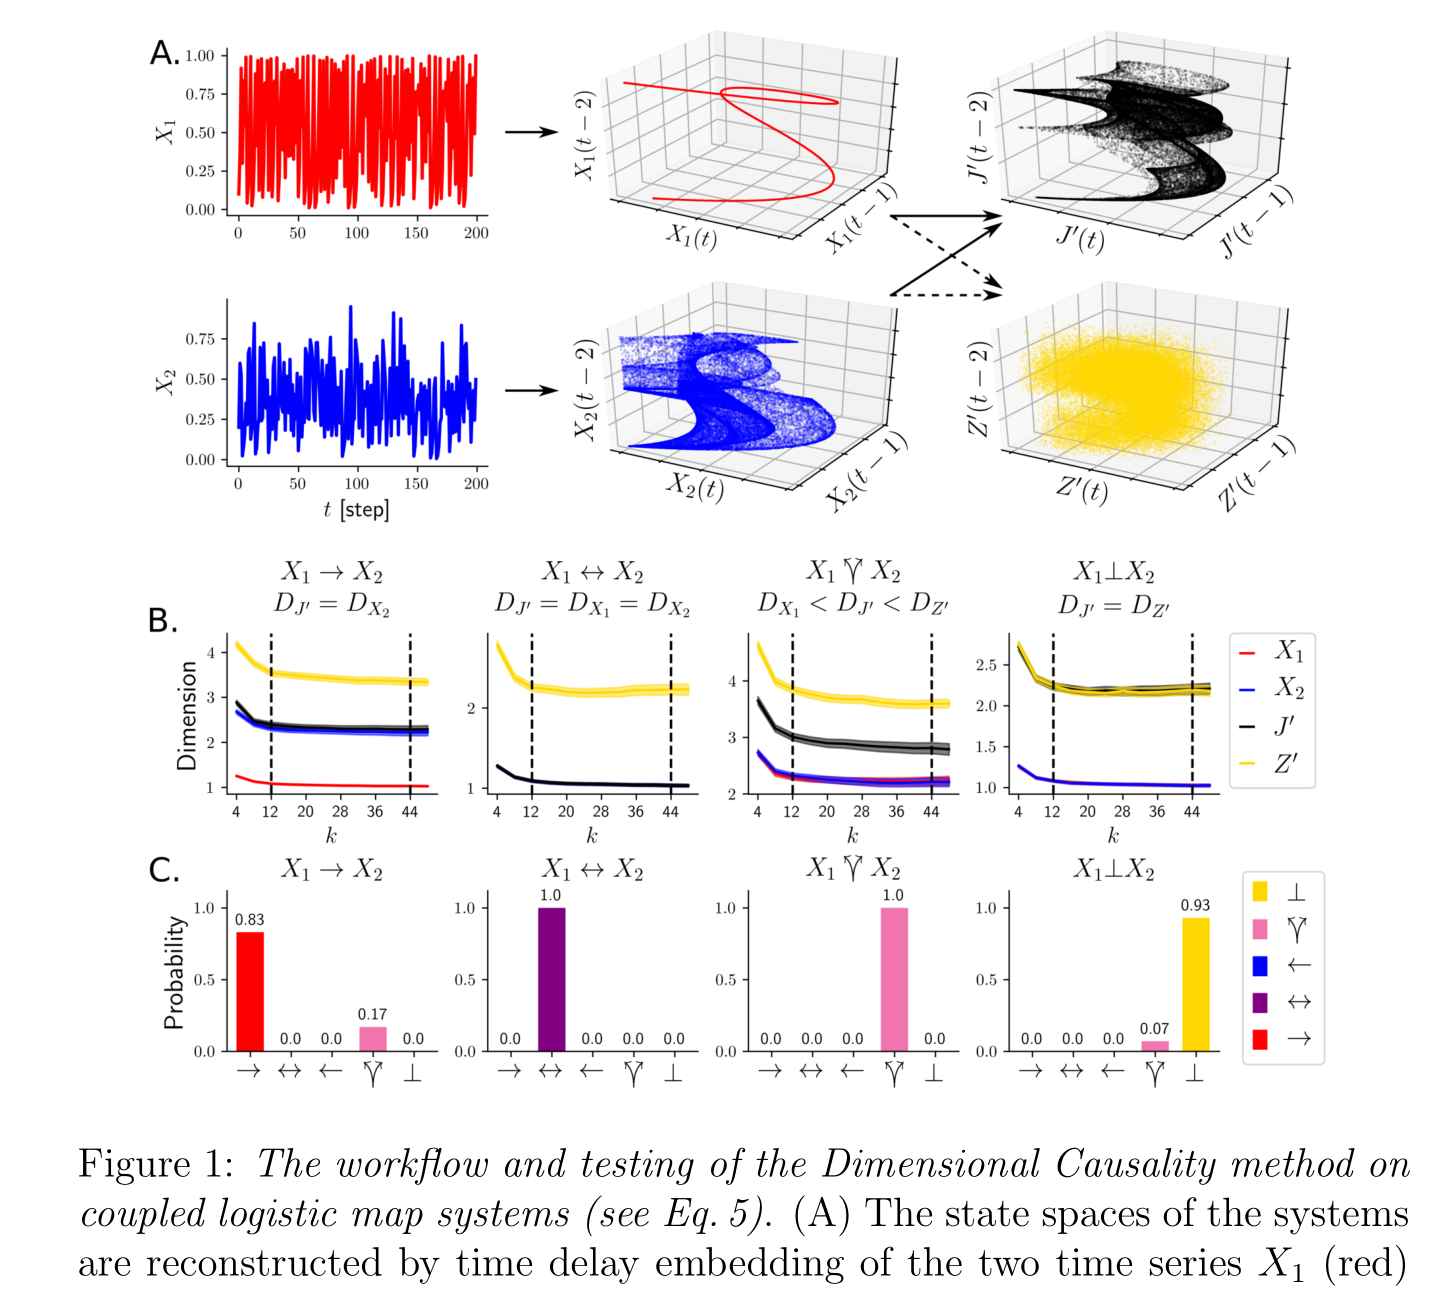
\includegraphics[scale=0.4]{figures/dimensional_causality.png}
    \caption{Dimensional Causality identifies a variety of causal structures. From \speccite{benkHo2018exact}.}
    \label{dim_cause}
\end{figure}

The also demonstrate their method on empirically obtained data and get interesting results. See scanned notes for more comments.

\begin{figure}[H]
    \centering
    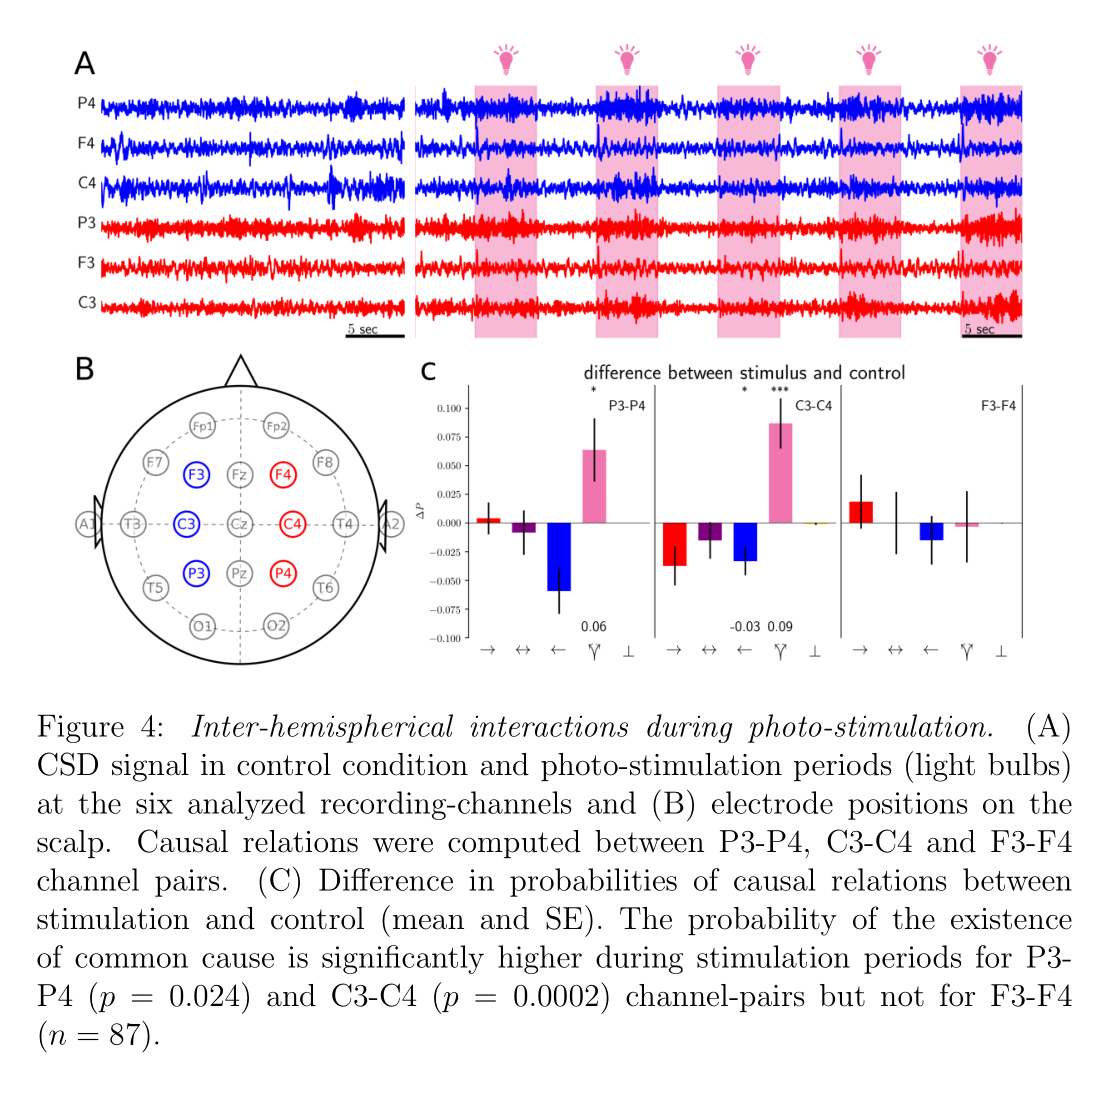
\includegraphics[scale=0.5]{figures/inter-hemispherical_interactions.png}
    \caption{An application of the technique of dimensional causality in \speccite{benkHo2018exact}.}
\end{figure}

\section{Other Noteworthy Articles}

In \speccite{wagner1999causality}, \citeauthor{wagner1999causality} argues that a ``...notion of causality can only only be meaningfully defined for systems with \textit{linear} interactions among their variables. For the vastly more important class of \textit{nonlinear} systems, no such notion is likely to exist.'' \\

In \speccite{white2011linking}, \citeauthor{white2011linking} use the formalism of \textit{settable systems}, a generalization of Pearl's Causal Models \parencite{pearl2000causality}, to closely link the concepts of Granger causality to that of Pearl causality.\\

At a quick glance, \speccite{blom2019beyond} appears to be doing a similar thing but for systems at a stable fixed point.\\

Also \speccite{arbach2015dynamic}.

\nocite{*}
\printbibliography
\end{document}
